\section{Register Pushdown Transducers and Register Pushdown Automata}
\subsection{Data words and registers}
We assume a countable set $D$ of \emph{data values}.
For finite alphabets $\Sigma_\dblI,\Sigma_\dblO$,
an infinite sequence $(a^\dblI_1,d_1)(a^\dblO,d'_1)\cdots \in ((\Sigma_\dblI\times D)\cdot(\Sigma_\dblO\times D))^\omega$ is called a \emph{data word}.
We let $\DW(\Sigma_\dblI,\Sigma_\dblO,D)=((\Sigma_\dblI\times D)\cdot(\Sigma_\dblO\times D))^\omega$.

For $k\in\Natz$, a mapping $\theta: [k] \to D$ is called an \emph{assignment}
(of data values to $k$ registers).
Let $\Theta_k$ denote the collection of assignments to $k$ registers.
We assume $\bot\in D$ as the initial data value and
let $\theta^k_\bot\in\Theta_k$ be the initial assignment such that
$\theta^k_\bot(i)=\bot$ for all $i\in[k]$.

% For $j_1\cdots j_n\in [k]^*$, we define $\theta(j_1\cdots j_n)=\theta(j_1)\cdots\theta(j_n)$ and $\theta(\varepsilon) = \varepsilon$.
We denote $\Tst_k = \scrP([k]\cup\{\top\})$ and $\Asgn_k = \scrP([k])$
where $\top\notin\Nat$ is a unique symbol that represents a stack top value.
$\Tst_k$ is the set of guard conditions.
For $\tst\in\Tst_k$, $\theta\in\Theta_k$ and $d,e\in D$,
we denote $(\theta,d,e)\models\tst$
if ($\theta(i) = d \Leftrightarrow i\in\tst$)
and ($e = d \Leftrightarrow \top\in\tst$) hold.
In the definitions of register pushdown transducer and automaton in the next section,
the data values $d$ and $e$ correspond to an input data value and a stack top data value, respectively.
$\Asgn_k$ is the set of assignment conditions.
For $\asgn\in\Asgn_k$, $\theta,\theta'\in\Theta_k$ and $d\in D$,
let $\theta[\asgn\leftarrow d]$ be the assignment
$\theta'$ such that $\theta'(i) = d$ for $i\in\asgn$ and $\theta'(i)=\theta(i)$ for $i\notin\asgn$.

\subsection{Register pushdown transducers}
\begin{definition}
A $k$-{register pushdown transducer} ($k$-RPDT) over finite alphabets $\Sigma_\dblI,\Sigma_\dblO$ and an infinite set $D$ of data values is
$\calT=(P, p_0, \Delta)$ where
$P$ is a finite set of states,
$p_0\in P$ is the initial state,
$\Delta: P\times\Sigma_\dblI\times\Tst_k \to P\times\Sigma_\dblO\times \Asgn_k \times [k]\times \Com([k])$ is a finite set of deterministic transition rules.
\end{definition}
$D$ is used as a stack alphabet.
For $u\in D^+$, $\theta'\in\Theta_k$ and $\com\in\Com([k])$, let us define $\upds(u,\theta',\com)$ as $\upds(u,\theta',\pop)=u(1:)$, $\upds(u,\theta',\skip)=u$ and $\upds(u,\theta',\push(j'))=\theta'(j')u$.
Let $\ID_\calT= P\times \Theta_k\times D^*$
and $\Rightarrow_\calT\ \subseteq \ID_\calT\times ((\Sigma_\dblI\times D)\cdot(\Sigma_\dblO\times D))\times \ID_\calT$ be the transition relation of $\calT$ such that $((p, \theta, u), (a,d^\dblI)(b,d^\dblO), (q, \theta', u'))\in\ \Rightarrow_\calT$ iff
there exists a rule $(p, a, \tst) \to (q, b, \asgn, j, \com) \in \Delta$
that satisfies the following conditions:
$(d^\dblI, u(0), \theta)\models\tst$, $\theta' = \theta[\asgn\leftarrow d^\dblI]$, $\theta'(j) = d^\dblO$ and
$u'=\upds(u,\theta',\com)$,
and we write $(p, \theta, u) \done_{\calT}^{(a,d^\dblI)(b,d^\dblO)}(q, \theta', u')$.
If $\calT$ is clear from the context,
we abbreviate
$\done_{\calT}^{(a,d^\dblI)(b,d^\dblO)}$ as $\done^{(a,d^\dblI)(b,d^\dblO)}$.
% If a sequence of IDs $(q_0, \theta_0, w_0), \cdots, (q_n, \theta_n, w_n)\in \ID_\mathcal{T}$
% and data values $d^\dblI_1, \cdots, d^\dblI_n, d^\dblO_1, \cdots, d^\dblO_n\in D$ satisfy $(q_{i-1}, \theta_{i-1}, w_{i-1})\done^{d^\dblI_i, d^\dblO_i}(q_i, \theta_i, w_i)$ for all $i\in[n]$, we write $(q_0, \theta_0, w_0)\done^{w^\dblI, w^\dblO}(q_n, \theta_n, w_n)$
% where $w^\dblI = d^\dblI_1 \cdots d^\dblI_n$ and $w^\dblO = d^\dblO_1 \cdots d^\dblO_n$.

% If we emphasize the rule $r$ and the data value $d$,
% we write $\done_d^r$.
A run and the language $L(\calT)$ of $\calT$ are those of deterministic $0$-TS $(\ID_\calT, (q_0,\theta^k_\bot, \bot), (\Sigma_\dblI\times D)\cdot(\Sigma_\dblO\times D), \emptyset, \Rightarrow_\calT, c)$ where $c(s)=2$ for all $s\in\ID_\calT$.
Let \RPDTk\ be the class of $k$-RPDT and \RPDT = $\bigcup_{k\in\Natz}$\RPDTk.
% Note that \RPDT$[0]$ = \PDT.

\begin{example}
\label{ex: PDT}
Let us consider $1$-RPDT
$\calT = (\{p,p'\},p,z_0,\Delta)$
over $\{a\},\{b\}$ and $\{z_0,z\}$ where
$\Delta = \{
(p, a, \tst) \rightarrow (p', b, \{1\}, 1, \push(1))
(p', a, \{\}) \rightarrow (p, b, \{1\}, 1, \push(1))
(p', a, \{1\}) \rightarrow (p, b, \{1\}, 1, \push(1))
(p, a, \{\top\}) \rightarrow (p', b, \{1\}, 1, \pop)
(p, a, \{1,\top\}) \rightarrow (p', b, \{1\}, 1, \pop)
\}$
Let $(\rho,w)\in \ID_\calT^\omega\times \{a,b\}^\omega$
be a pair of sequences where
$\rho=(p,z_0)(p,zz_0)(p,zzz_0)(p,zzzz_0)\cdots$ and $w=aba^\omega$,
then $(\rho,w)$ is a run of $\calT$.

Let $\#_a(w), \#_b(w)\in \Natz$ denote the number of $a$, $b$
appearing in $w\in\{a,b\}^*$, respectively.
$L(\calT)$ is the set of the sequence $w\in \{a,b\}^\omega$
that satisfies one of the following conditions:
(i) $w = t_0 w_0 t_1 w_1\cdots
\in(\{ab, ba\} \times \{aa, bb\}^*)^\omega$
where for all $i\geq 0$, $t_i\in \{ab, ba\}$ and
$w_i\in \{aa, bb\}^*$ such that
$\#_b(w_i)-\#_a(w_i)=2$.
(ii) $w = t_0 w_0 t_1 w_1\cdots t_n w_n
\in(\{ab, ba\} \times \{aa, bb\}^*)^*\cdot(\{ab, ba\} \times \{aa, bb\}^\omega)$
where for all $0\leq i\leq n$, $t_i\in \{ab, ba\}$ and
$w_i\in \{aa, bb\}^*$ such that
$\#_b(w_i)-\#_a(w_i)=2$ for $0\leq i< n$ and
$w_n\in \{aa, bb\}^\omega$ such that
$\#_a(w')-\#_b(w')\geq 0$
for all subsequence $w'=w(0:m)$ of $w$ for all $m\in\Natz$.
\begin{figure}[t]
  \centering
  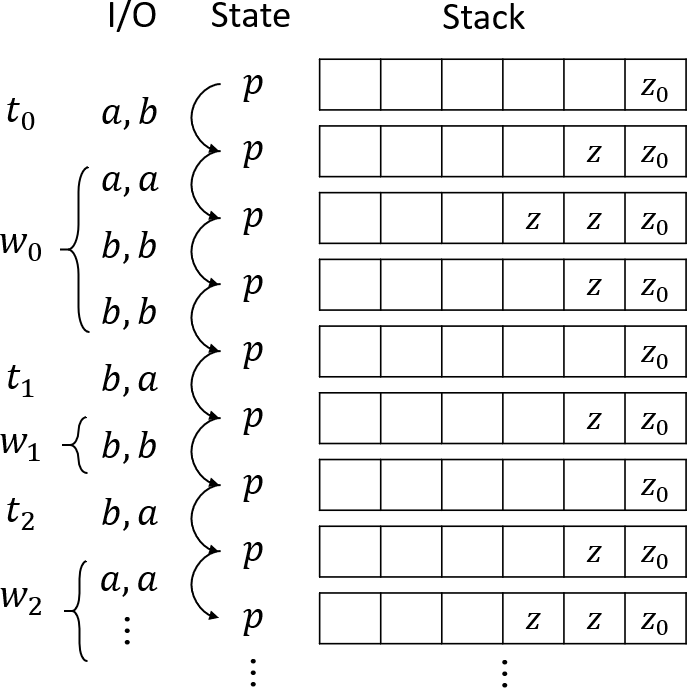
\includegraphics[width=6cm]{PDT.png}
  \caption{An example of run for a sequence $w = t_0 w_0 t_1 w_1\cdots$.}
  \label{fig: PDT}
\end{figure}
\end{example}



\subsection{Register pushdown automata}\label{sec:RA}
\begin{definition}
A nondeterministic $k$-register pushdown automaton ($k$-NRPDA) over $\Sigma_\dblI,\Sigma_\dblO$ and $D$ is $\calA=(Q, Q_\dblI, Q_\dblO, q_0, \delta, c)$, where
\begin{itemize}
\item $Q$ is a finite set of states,
\item $Q_\dblI\cup Q_\dblO = Q, Q_\dblI\cap Q_\dblO = \emptyset$,
\item $q_0\in Q$ is the initial state, and
\item $\delta: Q \times (\Sigma\cup\{\tau\})\times \Tst_k \to \scrP(Q \times\Asgn_k\times \Com([k]))$ is a transition function having one of the forms:
\begin{itemize}
\item $(q_\dblX,a_\dblX,\tst)\to(q_\overX,\asgn,\com)$ (input/output rule)
\item $(q_\dblX,\tau,\tst)\to(q'_\dblX,\asgn,\com)$ ($\tau$ rule)
\end{itemize}
where $(\dblX, \overX)\in\{(\dblI, \dblO), (\dblO,\dblI)\}$,
$q_\dblX, q'_\dblX\in Q_\dblX, q_\overX\in Q_\overX, a_\dblX\in \Sigma_\dblX$, $\tst\in\Tst_k$, $\asgn\in\Asgn_k$ and $\com\in\Com([k])$.
\item $c: Q \to [n]$ where $n\in \Nat$ is the number of priorities.
\end{itemize}
\end{definition}
\noindent
Let $\ID_\calA= Q\times \Theta_k\times D^*$.
We define the transition relation $\vdash_\calA\ \subseteq\ID_\calA\times ((\Sigma\cup\{\tau\})\times D)\times \ID_\calA$ as
$((q,\theta,u), (a,d), (q',\theta',u'))\in\ \vdash_\calA$,
written as $(q,\theta,u)\vdash^{(a,d)}(q',\theta',u')$, iff
there exists a rule $(p, a, \tst) \to (q, \asgn, \com) \in \delta$
such that
$(d, u(0), \theta)\models\tst$, $\theta' = \theta[\asgn\leftarrow d]$ and
$u'= \upds(u,\theta',\com)$.
We write $\vdash^{(a,d)}_\calA$ as $\vdash^{(a,d)}$ if $\calA$ is clear from the context.
For $s,s'\in\ID_\calA$ and
$w\in((\Sigma_\dblI\times D)\cdot (\Sigma_\dblO\times D))^{m}$,
we write $s\vdash^{w}s'$ if
there exists $\rho\in\ID_\calA^{m+1}$ such that
$\rho(0)=s, \rho(m)=s'$, and
$\rho(0)\vdash^{w(0)}\cdots\vdash^{w(m-1)}\rho(m)$.

A run and the language $L(\calA)$ of $k$-DRPDA $\calA$ are those of TS
$\calS_\calA=(\ID_\calA, (q_0, \theta^k_\bot, \bot), \Sigma\times D, \{\tau\}\times D, \Rightarrow_\calA, c')$ where
$c'((q,\theta,u))=c(q)$ for all $(q,\theta,u)\in\ID_\calA$.
We call an $\calA$ deterministic, or $k$-DRPDA, if $\calS_\calA$ is deterministic.
We call an $\calA$ $(m,k)$-NRPDA (or an $(m,k)$-DRPDA when $\calA$ is deterministic)
if $\calS_\calA$ is an $m$-TS.
We abbreviate $(0,k)$-NRPDA ($(0,k)$-DPDA) as $k$-NRPDA ($k$-DRPDA).
